% Copyright (c) 2026 CorrectBrain
% SPDX-License-Identifier: MIT

\PassOptionsToPackage{dvipsnames,svgnames,x11names}{xcolor}
\documentclass[tikz,border=8pt]{standalone}
\usetikzlibrary{arrows.meta,positioning,calc,shapes,shadows,decorations.pathmorphing,shapes.geometric,backgrounds,decorations.markings,decorations.pathreplacing,decorations.text,fit,shapes.misc,shapes.arrows,matrix,bending,3d,chains,intersections,shapes.symbols,svg.path,shapes.multipart,snakes,shapes.callouts,angles,quotes}
\usetikzlibrary{fadings,shadows.blur,patterns,patterns.meta}
\usepackage{amsmath}
\usepackage{amssymb}
\usepackage{fontawesome5}

\providecolor{gold}{RGB}{212,175,55}
\providecolor{silver}{RGB}{192,192,192}
\providecolor{bronze}{RGB}{205,127,50}
\providecolor{darkblue}{RGB}{0,0,139}
\providecolor{lightblue}{RGB}{173,216,230}
\providecolor{darkgreen}{RGB}{0,100,0}
\providecolor{lightgreen}{RGB}{144,238,144}
\providecolor{darkred}{RGB}{139,0,0}
\providecolor{navy}{RGB}{0,0,128}
\providecolor{skyblue}{RGB}{135,206,235}
\providecolor{beige}{RGB}{245,245,220}
\providecolor{cream}{RGB}{255,253,208}

% --- POSTGRADUATE COLOR PALETTE ---
\definecolor{imgblue}{RGB}{41, 128, 185}
\definecolor{contgray}{RGB}{208, 211, 212}
\definecolor{darktext}{RGB}{44, 62, 80}
\definecolor{ceilpurple}{RGB}{142, 68, 173}
\definecolor{macred}{RGB}{235, 96, 92}
\definecolor{macyellow}{RGB}{247, 192, 43}
\definecolor{macgreen}{RGB}{46, 203, 112}

\begin{document}
\begin{tikzpicture}

% Canvas Background Rule
\fill[white] (-10.1997,-8.563) rectangle (10, 19);

% ==========================================
% GLOBAL HEADER
% ==========================================
\node[font=\Huge\bfseries\color{darktext}] at (0, 17.5) {Viewport Scenarios: The Ceiling in Action};
\node[font=\large\color{darktext!80}] at (0, 16.8) {Precise Mathematical Rendering (Scale: 1 unit = 100px)};

% ==========================================
% SCENARIO 1: DESKTOP (Wide Container)
% ==========================================
\node[font=\Large\bfseries\color{darktext}, anchor=west] at (-6, 15.5) {\faDesktop\ \ 1. Desktop Viewport ($W_{\text{container}} = 1200\text{px}$)};
\node[font=\normalsize\color{darktext!70}, anchor=west, text width=15cm, align=left] at (-6, 14.8) {$1200\text{px} > 800\text{px}$. Ceiling activated. Image refuses to stretch, centering logic applies.};

% Browser Window (Width 12 units = 1200px, Content Height 4 units = 400px)
\fill[white, draw=contgray!50, thick, blur shadow={shadow blur steps=10, shadow opacity=15, shadow yshift=-2pt}] (-6, 9.2) rectangle (6, 14.0);
\fill[contgray!20, draw=contgray!50, thick] (-6, 13.2) rectangle (6, 14.0);
\fill[white, draw=contgray!40, rounded corners=3pt] (-4.3, 13.35) rectangle (5.5, 13.85);

% Realistic macOS Window Buttons (3D Shading)
\shade[inner color=macred!50, outer color=macred] (-5.6, 13.6) circle (3.5pt);
\shade[inner color=macyellow!50, outer color=macyellow] (-5.2, 13.6) circle (3.5pt);
\shade[inner color=macgreen!50, outer color=macgreen] (-4.8, 13.6) circle (3.5pt);

% URL Bar Container Text
\node[font=\small\bfseries\color{darktext!70}] at (0.6, 13.6) {Container Width: 1200px};

% Rendered Image Box (8 units wide, 4 units high)
\fill[imgblue!15, draw=imgblue, thick, blur shadow={shadow blur steps=8, shadow opacity=15, shadow yshift=-1.5pt}] (-4, 9.2) rectangle (4, 13.2);
\node[font=\Huge\color{imgblue!60}] at (0, 11.9) {\faImage};
\node[font=\large\bfseries\color{imgblue}] at (0, 11.0) {Rendered: 800px $\times$ 400px};
\node[font=\normalsize\bfseries\color{ceilpurple}, fill=white, inner sep=2pt, rounded corners=2pt] at (0, 10.1) {$\mathbf{W_{\text{render}} = \min(800, 1200) = 800}$};

% Ceiling Halt Arrows & Labels
\draw[-Stealth=3mm, line width=2pt, ceilpurple] (-6, 11.2) -- (-4.1, 11.2);
\node[font=\scriptsize\bfseries\color{ceilpurple}, fill=white, inner sep=1.5pt, above, yshift=2pt] at (-5.05, 11.2) {Ceiling Halt};
\node[font=\tiny\color{ceilpurple}, below, yshift=-2pt] at (-5.05, 11.2) {(Empty Space)};

\draw[-Stealth=3mm, line width=2pt, ceilpurple] (6, 11.2) -- (4.1, 11.2);
\node[font=\scriptsize\bfseries\color{ceilpurple}, fill=white, inner sep=1.5pt, above, yshift=2pt] at (5.05, 11.2) {Ceiling Halt};
\node[font=\tiny\color{ceilpurple}, below, yshift=-2pt] at (5.05, 11.2) {(Empty Space)};


% ==========================================
% SCENARIO 2: TABLET (Narrow Container)
% ==========================================
\node[font=\Large\bfseries\color{darktext}, anchor=west] at (-6, 7.5) {\faIcon{tablet-alt}\ \ 2. Tablet Viewport ($W_{\text{container}} = 600\text{px}$)};
\node[font=\normalsize\color{darktext!70}, anchor=west, text width=15cm, align=left] at (-6, 6.8) {$600\text{px} < 800\text{px}$. Ceiling enforced. Image mathematically forced to scale down to fit container.};

% Intrinsic Ghost Image (8 units wide, 4 units high, top-aligned at y=5.2)
\draw[macred!80, dashed, dash pattern=on 6pt off 4pt, line width=1.5pt, fill=macred!5] (-4, 1.2) rectangle (4, 5.2);

% Browser Window (Width 6 units = 600px, Content Height 3 units = 300px)
\fill[white, draw=contgray!50, thick, blur shadow={shadow blur steps=10, shadow opacity=15, shadow yshift=-2pt}] (-3, 2.2) rectangle (3, 6.0);
\fill[contgray!20, draw=contgray!50, thick] (-3, 5.2) rectangle (3, 6.0);
\fill[white, draw=contgray!40, rounded corners=2.5pt] (-1.4, 5.35) rectangle (2.8, 5.85);

% Realistic macOS Window Buttons (3D Shading)
\shade[inner color=macred!50, outer color=macred] (-2.6, 5.6) circle (3pt);
\shade[inner color=macyellow!50, outer color=macyellow] (-2.2, 5.6) circle (3pt);
\shade[inner color=macgreen!50, outer color=macgreen] (-1.8, 5.6) circle (3pt);

% URL Bar Container Text
\node[font=\footnotesize\bfseries\color{darktext!70}] at (0.7, 5.6) {Container: 600px};

% Rendered Image Box (6 units wide, 3 units high) - Drawn over Ghost
\fill[imgblue!15, draw=imgblue, thick, blur shadow={shadow blur steps=8, shadow opacity=15, shadow yshift=-1.5pt}] (-3, 2.2) rectangle (3, 5.2);
\node[font=\huge\color{imgblue!60}] at (0, 4.1) {\faImage};
\node[font=\normalsize\bfseries\color{imgblue}] at (0, 3.4) {Rendered: 600px $\times$ 300px};
\node[font=\small\bfseries\color{ceilpurple}, fill=white, inner sep=2pt, rounded corners=2pt] at (0, 2.7) {$\mathbf{W_{\text{render}} = \min(800, 600) = 600}$};

% Intrinsic Label (Bottom-center with white fill to prevent overlap)
\node[font=\scriptsize\bfseries\color{macred}, fill=white, inner sep=2pt, rounded corners=2pt] at (0, 1.2) {Intrinsic: 800px $\times$ 400px};

% Squeeze / Compression Arrows strictly pushing from Intrinsic to Container boundary
\draw[-Stealth=3mm, line width=2pt, ceilpurple] (-4, 3.7) -- (-3.1, 3.7);
\node[font=\scriptsize\bfseries\color{ceilpurple}, above, yshift=2pt, fill=white, inner sep=1.5pt] at (-3.55, 3.7) {Scale to Fit};

\draw[-Stealth=3mm, line width=2pt, ceilpurple] (4, 3.7) -- (3.1, 3.7);
\node[font=\scriptsize\bfseries\color{ceilpurple}, above, yshift=2pt, fill=white, inner sep=1.5pt] at (3.55, 3.7) {Scale to Fit};


% ==========================================
% SCENARIO 3: MOBILE (Very Narrow Container)
% ==========================================
\node[font=\Large\bfseries\color{darktext}, anchor=west] at (-6.0228,-0.9569) {\faIcon{mobile-alt}\ \ 3. Mobile Viewport ($W_{\text{container}} = 300\text{px}$)};
\node[font=\normalsize\color{darktext!70}, anchor=west, text width=15cm, align=left] at (-6.0228,-1.6569) {$300\text{px} \ll 800\text{px}$. \texttt{height: auto} strictly preserves the intrinsic 2:1 aspect ratio on vertical axes.};

% Intrinsic Ghost Image (8 units wide, 4 units high, top-aligned at y=-3.4)
\draw[macred!80, dashed, dash pattern=on 6pt off 4pt, line width=1.5pt, fill=macred!5] (-4, -7.4) rectangle (4, -3.4);

% Browser Window (Width 3 units = 300px, Content Height 1.5 units = 150px)
\fill[white, draw=contgray!50, thick, blur shadow={shadow blur steps=10, shadow opacity=15, shadow yshift=-2pt}] (-1.5, -4.9) rectangle (1.5, -2.6);
\fill[contgray!20, draw=contgray!50, thick] (-1.5, -3.4) rectangle (1.5, -2.6);

% Realistic macOS Window Buttons (Standardized 0.8 Height UI)
\shade[inner color=macred!50, outer color=macred] (-1.2, -3.0) circle (2.5pt);
\shade[inner color=macyellow!50, outer color=macyellow] (-0.9, -3.0) circle (2.5pt);
\shade[inner color=macgreen!50, outer color=macgreen] (-0.6, -3.0) circle (2.5pt);
\fill[white, draw=contgray!40, rounded corners=1.5pt] (-0.3, -3.25) rectangle (1.4, -2.75);
\node[font=\fontsize{4.5}{5.5}\selectfont\bfseries\color{darktext!70}, anchor=center] at (0.55, -3.0) {Container: 300px};

% Rendered Image Box (3 units wide, 1.5 units high) - Drawn over Ghost
\fill[imgblue!15, draw=imgblue, thick, blur shadow={shadow blur steps=6, shadow opacity=15, shadow yshift=-1pt}] (-1.5, -4.9) rectangle (1.5, -3.4);
\node[font=\small\color{imgblue!60}] at (0, -3.9) {\faImage};
\node[font=\fontsize{6}{7}\selectfont\bfseries\color{imgblue}] at (0, -4.35) {300px $\times$ 150px};
\node[font=\fontsize{6}{7}\selectfont\bfseries\color{ceilpurple}, fill=white, inner sep=0.5pt, rounded corners=1pt] at (0, -4.7) {$\mathbf{W_{\text{render}} = \min(800, 300) = 300}$};

% Intrinsic Label (Bottom-center with white fill)
\node[font=\scriptsize\bfseries\color{macred}, fill=white, inner sep=2pt, rounded corners=2pt] at (0, -7.4) {Intrinsic: 800px $\times$ 400px};

% Squeeze / Compression Arrows strictly pushing from Ghost boundary to Container boundary
\draw[-Stealth=3mm, line width=2pt, ceilpurple] (-4, -4.15) -- (-1.6, -4.15);
\node[font=\scriptsize\bfseries\color{ceilpurple}, above, yshift=2pt, fill=white, inner sep=1.5pt] at (-2.8, -4.15) {Scale to Fit};

\draw[-Stealth=3mm, line width=2pt, ceilpurple] (4, -4.15) -- (1.6, -4.15);
\node[font=\scriptsize\bfseries\color{ceilpurple}, above, yshift=2pt, fill=white, inner sep=1.5pt] at (2.8, -4.15) {Scale to Fit};

\end{tikzpicture}
\end{document}
